\section{Evaluating Information Retrieval}
\label{sec:EvaluatingInformationRetrieval}

In this section, we will use the standard terminology to denote whether the classification is correct (true) or not (false), for both positive and negative categories, as given by the confusion matrix (\tabletext{}~\ref{tab:ConfusionMatrix}).

\begin{table}[t]
    \centering

    \begin{tabular}{c|cc}
        \toprule
                                        & \tblcolname{Actual positive} & \tblcolname{Actual negative} \\
        \cline{2-3}
        \tblcolname{Predicted positive} & \gls{tp}                     & \gls{fp}                     \\
        \cline{2-3}
        \tblcolname{Predicted negative} & \gls{fn}                     & \gls{tn}                     \\
        \bottomrule
    \end{tabular}

    \caption[Confusion matrix]{A confusion matrix in the standard form.}
    \label{tab:ConfusionMatrix}
\end{table}

% ##############################################################################
\subsection{Evaluating Bounding Box Prediction}
\label{ssec:EvaluatingBoundingBoxPrediction}

\subsubsection{Intersection Over Union}
\label{sssec:IntersectionOverUnion}

\glslocalreset{iou}

\gls{iou} measures the overlap between two \glspl{bbox}. Let $\subsup{\vect{b}}{1}{T} = \sbrackets{x_1, y_1, w_1, h_1}$ and $\subsup{\vect{b}}{2}{T} = \sbrackets{x_2, y_2, w_2, h_2}$ be two \glspl{bbox} described by vectors containing $4$ elements. The respective elements are given by $x$, $y$ coordinates of the top-left corner and the \gls{bbox} width and height. The intersection area between $\vect{b}_1$ and $\vect{b}_2$ is defined as
\begin{equation}
    \begin{aligned}
        \vect{b}_1 \cap \vect{b}_2 =
         & \max \cbrackets{0,
            \min \cbrackets{x_1 + w_1, x_2 + w_2} - \max \cbrackets{x_1, x_2} + 1}
        \times                \\
         & \max \cbrackets{0,
            \min \cbrackets{y_1 + h_1, y_2 + h_2} - \max \cbrackets{y_1, y_2} + 1},
    \end{aligned}
\end{equation}
and the area of their union is given by
\begin{equation}
    \vect{b}_1 \cup \vect{b}_2 = w_1 h_1 + w_2 h_2 - \vect{b}_1 \cap \vect{b}_2.
\end{equation}
Then, the final \gls{iou} metric between $\vect{b_1}$ and $\vect{b_2}$ is computed as (\figtext{}~\ref{fig:IntersectionOverUnion})
\begin{equation}
    \label{eq:IntersectionOverUnion}
    \func{\IOU}{\vect{b}_1, \vect{b}_2} =
    \frac{\vect{b}_1 \cap \vect{b}_2}{\vect{b}_1 \cup \vect{b}_2},
\end{equation}
where $0 \leq \func{\IOU}{\vect{b}_1, \vect{b}_2} \leq 1$, such that value of $0$ represents no intersection, while value of $1$ represents a complete overlap. In terms of object detection or object tracking evaluation, an \gls{iou} threshold, $t$, such that $0 \leq t \leq 1$, can be associated with this metric, denoting the decision boundary whether the prediction is a \gls{tp} or a \gls{fp}.

% ------------------------------------------------------------------------------
\begin{figure}[t]
    \centerline{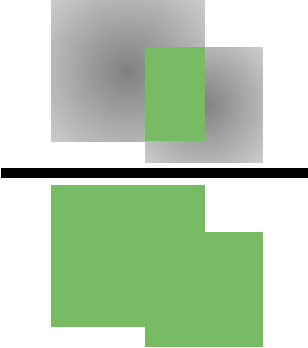
\includegraphics[width=0.2\linewidth]{figures/theoretical_foundations/intersection_over_union.pdf}}
    \caption[\gls{iou} visualization]{Computation of the \gls{iou} metric between two \glspl{bbox} using of ratio of the area of overlap and the area of the union.}
    \label{fig:IntersectionOverUnion}
\end{figure}
% ------------------------------------------------------------------------------

% ##############################################################################
\subsection{Mean Average Precision}
\label{ssec:MeanAveragePrecision}

\glslocalreset{map}

\gls{map} is commonly used for evaluation of tracking algorithms, document searching systems, object detection, object \gls{reid}, and many others. Generally speaking, it measures the success rate of an information retrieval algorithm.

\subsubsection{Object Re-Identification}
\label{sssec:ObjectReIdentification}

A common use case in the context of object \gls{reid} is to use \gls{map} to assess the search results for a particular query using Euclidean distance or cosine similarity as a metric. Oftentimes the model is trained with the intent to use one of these trivial metrics. Furthermore, this approach is often paired with \emph{top-k} accuracy, typically \emph{top-1}, \emph{top-2} and \emph{top-5}.

In a typical \gls{reid} evaluation setup, there is a query set and a gallery set. For each object in the query set the aim is to retrieve a similar identity from the gallery set. The computation of the \gls{ap} for a query image $q$ is thus defined as
\begin{equation}
    \label{eq:AveragePrecision}
    \func{\AP}{q} = \frac{1}{\func{N_{gt}}{q}} \sum_{k} \func{P}{k} \times {\delta}_k,
\end{equation}
where $\func{P}{k}$ represents precision at rank $k$, $\func{N_{gt}}{q}$ is the total number of true retrievals for the query $q$. The indicator ${\delta}_k$ is equal to $1$ when the matching of query image $q$ to a test image is correct at rank $r$, such that $1 \leq r \leq k$. The \gls{map} is then calculated as average over all query images, concretely
\begin{equation}
    \label{eq:MeanAveragePrecision}
    \MAP = \frac{1}{Q} \sum_q \func{\AP}{q},
\end{equation}
where $Q$ is the total number of query images, as described in~\cite{kuma2019vehiclereid}. \eqtext{}~\ref{eq:MeanAveragePrecision} essentially tells us that, for a given query $q$, we calculate its corresponding \gls{ap} (defined in \eqtext{}~\ref{eq:AveragePrecision}), and then take the mean of the all these \gls{ap} scores, quantifying how well our model responds to queries on average.

\subsubsection{Object Detection}

Object detectors seek to identify the presence of objects in images. The evaluation metric of such a model has to take the \gls{bbox} prediction into account, as there can be just a partial overlap of the predicted \gls{bbox} with the ground truth one. The previously defined \gls{map} is also used for object detection~\cite{everingham2010pascalvoc}.

In a ranked retrieval context, appropriate sets of retrieved documents are naturally given by the \emph{top-k} retrieved documents and for each such set, the precision-recall curve can be plotted. With this in mind, recall is defined as the proportion of all positive examples ranked above a given rank. Precision is the proportion of all examples above that rank which are from the positive class. In~\cite{everingham2010pascalvoc}, the \gls{ap} is computed for $11$ equally spaced discrete recall levels, specifically $\sbrackets{0.0, 0.1, 0.2, \dots, 1.0}$, using
\begin{equation}
    \AP = \frac{1}{11} \sum_{r \in \cbrackets{0.0, 0.1, \dots, 1.0}} \func{p_{interp}}{r},
\end{equation}
where the precision at each recall level $r$ is interpolated by taking the maximum precision measured for a method for which the corresponding recall exceeds $r$. Precision interpolation is used to remove the \emph{zig-zag} pattern by evaluating
\begin{equation}
    \func{p_{interp}}{r} = \underset{\tilde{r}:\tilde{r} \geq r}{\max} \quad \func{p}{\tilde{r}},
\end{equation}
with $\func{p}{\tilde{r}}$ representing the measures precision at a specific recall level $\tilde{r}$~\cite{salton1983introduction}.
